
\begin{question}
Solve the system of equations.

\[\begin{aligned}
- x^{2} + 2 x + y &= 38 \\
6 x - y &= -29
\end{aligned}\]
\end{question}

\begin{solution}
There is one solution.

\[(-3,11)\]

This system represents a parabola and a tangent line.

\begin{figure}
\centering
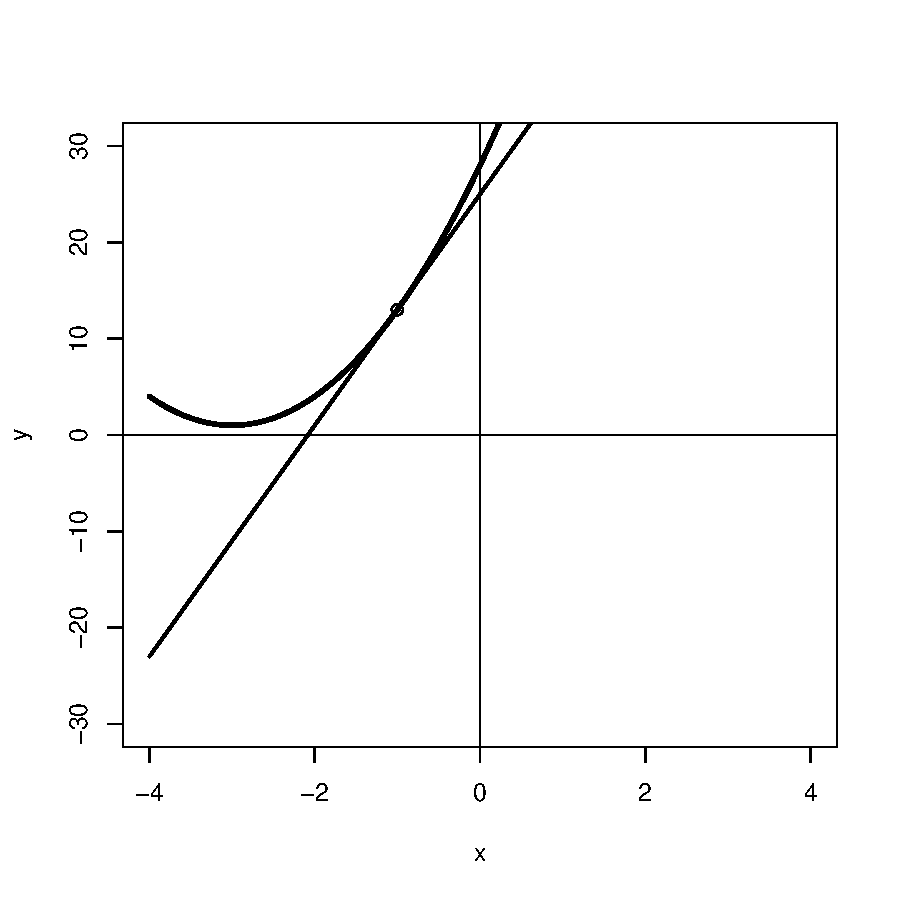
\includegraphics{unnamed-chunk-2-1-2.pdf}
\caption{plot of chunk unnamed-chunk-2}
\end{figure}
\end{solution}

